\documentclass[12pt,twoside]{article}
\usepackage[spanish,es-tabla]{babel}
\usepackage[a4paper]{geometry}

\usepackage{graphicx}               % Para incluir imágenes
\usepackage{amsmath}                % Para el manejo de matemáticas
\usepackage{url}
\usepackage{array}					% Para ajustar el texto en la celda
\usepackage{tabularx}
\usepackage{lipsum}
\usepackage{enumitem}
\usepackage{listings}
\usepackage{xcolor}
\usepackage{algorithm}
\usepackage{algpseudocode}
\usepackage{amssymb}

\lstdefinestyle{pythonstyle}{
	language=Python,
	basicstyle=\ttfamily\small,
	keywordstyle=\color{blue}\bfseries,
	commentstyle=\color{gray},
	stringstyle=\color{red},
	numbers=left,
	numberstyle=\tiny,
	stepnumber=1,
	frame=single,
	backgroundcolor=\color{lightgray!20},
	tabsize=4,
	showstringspaces=false,
	breaklines=true,        % Permite que las líneas largas se dividan
	linewidth=\linewidth    % Autoajuste al ancho del contenedor
}

% Opening
\title{Solución de problemas mediante recocido simulado}
\author{Erick Jesse Angeles López}


% Definir un comando para palabras clave
\newcommand{\keywords}[1]{%
	\begin{center}
		\textbf{Palabras clave:} #1
	\end{center}
}

\renewcommand{\baselinestretch}{1}
\setcounter{page}{1}
\setlength{\textheight}{21.6cm}
\setlength{\textwidth}{14cm}
\setlength{\oddsidemargin}{1cm}
\setlength{\evensidemargin}{1cm}
\pagestyle{myheadings}
\thispagestyle{empty}
\markboth{\small{Ángeles López Erick Jesse}}{\small{Solución de problemas mediante recocido simulado}}
\date{}

\begin{document}
	
	\begin{center}
		
		% Contenido izquierdo - Imagen
		\begin{minipage}{0.17\textwidth}
			\centering
			
\includegraphics[width=0.7\textwidth]{img/cic_logo.png} % Ajusta esta línea
		\end{minipage}
		\begin{minipage}{.55\textwidth}
			\centering
			{\Large Instituto Politécnico Nacional}\\
			{\Large Escuela Superior de Cómputo}\\
			{\Large Centro de Investigación en Computación}
		\end{minipage}
		\begin{minipage}{0.17\textwidth}
			\centering
			
\includegraphics[width=0.9\textwidth]{img/escom_logo} % Ajusta esta línea
		\end{minipage}			
	\end{center}
	
	
	\centerline{\bf Ingeniería en Inteligencia Artificial, Metaheuristicas}
	
	\centerline{\bf Fecha: \today}
	
	\centerline{}
	
	%\centerline{}
	
	
	\begin{center}
		\Large{\textsc{Recocido simulado}} 
	\end{center}
	\centerline{}
	\centerline{\bf {\textit{Presenta}}}
	\centerline{}
	\centerline{\bf {Angeles López Erick Jesse\footnote{eangelesl1700@alumno.ipn.mx}}}
	\centerline{}
	\centerline{}
	\centerline{\bf {Disponible en:}}
	\centerline{\text{\url{github.com/JesseAngeles/Metaheuristicas}}}
	
	
	
	\newtheorem{Theorem}{\quad Theorem}[section]
	
	\newtheorem{Definition}[Theorem]{\quad Definition}
	
	\newtheorem{Corollary}[Theorem]{\quad Corollary}
	
	\newtheorem{Lemma}[Theorem]{\quad Lemma}
	
	\newtheorem{Example}[Theorem]{\quad Example}
	
	\bigskip
	
	\bigskip
	
	\begin{abstract} 
		Se describe el comportamiento del algoritmo \textit{Simulated Annealing} para resolver problemas de optimización local. Se estudia el comportamiento del algoritmo, ventajas y desventanas, pseudocodigo, comparativa con \textit{RMHC} y propuestas para resolver problemas en computación como \textit{Knapsack problem} y \textit{Travel Salesman problem}.
	\end{abstract}
	
	\keywords{Algoritmo, Pseudocódigo, Resultado óptimo, Simulated Annealing}
	
	\clearpage
	
	\tableofcontents
	\clearpage
		
	\section{Simulated Annealing}

	\subsection{Recocido físico}

	Trabajar con los metales en sus estados puros puede resultar contraproducente. Se busca obtener las propiedades deseadas mediante diferentes tratamientos, entre ellos, el recocido (\textit{Annealing}).
	
	Este proceso térmico busca cambiar las propiedades físicas y mecánicas del material con el objetivo de volverlo mas trabajable \cite{recocido}.

	Este proceso calienta un metal (como el acero) a altas temperaturas para enfriarlo lentamente con el objetivo de eliminar defectos estructurales, como tensiones internas, que pudieron haber aparecido en procesos de deformación o de enfriamiento rápido. Este enfriamiento permite que los átomos se reorganicen en una configuración mas estable y de menor energía \cite{recocido_2}.
	
	\subsection{Recocido simulado}

	El recocido simulado (\textit{Simulated Annealing}) se inspira del recocido físico pero aplicado a un contexto matemático. Se busca resolver problemas de optimización mediante un proceso de exploración del espacio de soluciones.
	
	Se compone de cinco elementos:
	\begin{itemize}
		\item \textbf{Solución inicial}: Se comienza con una solución inicial aleatoria o previamente determinada por el problema
		
		\item \textbf{Energía}: Se define una función objetivo (de energía) que mide la calidad de la solución. Esta función es única para cada problema de optimización (máximos y mínimos).
		
		\item \textbf{Enfriamiento}: Se sigue un proceso análogo al enfriamiento controlado. En cada iteración se genera una nueva solución vecina a partir de la solución actual. 
		
		\begin{itemize}
			\item Si la nueva solución es \textbf{mejor} se acepta como la solución actual.
			\item Si la nueva solución es \textbf{peor}, la decisión de aceptarla depende de una probabilidad (la probabilidad disminuye gradualmente conforme avanza el proceso).
		\end{itemize}
		
		A temperaturas altas se permiten cambios grandes de enfriamiento, pero a medida que el sistema se ``enfría'' la probabilidad de que una solución peor sea aceptada disminuye.
		
		\item \textbf{Temperatura}: Probabilidad de aceptar peores soluciones. Inicia alta y decrece en cada iteración (decrecimiento lineal, exponencial, factorial, etc).
		
		\item \textbf{Convergencia}: El algoritmo se detiene en una temperatura aceptable o se alcanzo un máximo de iteraciones sin encontrar mejoras significativas.
	\end{itemize}
	\subsection{Ventajas}
	
	\begin{itemize}
		\item \textbf{Versatilidad}: El \textit{Simulated Annealing} no requiere un conocimiento previo del problema, lo que lo convierte en un algoritmo versátil, aplicable a una amplia gama de problemas de optimización.
		
		\item \textbf{Exploración eficaz}: Gracias a su capacidad de escapar de óptimos locales, el algoritmo permite explorar el espacio de soluciones y aumenta la probabilidad de encontrar soluciones globales óptimas.
		
		\item \textbf{Facilidad de implementación}: El algoritmo es relativamente sencillo de implementar, ya que no requiere operaciones complejas como derivadas ni grandes cantidades de datos. Los cálculos son directos y accesibles.
	\end{itemize}
	
	\subsection{Desventajas}
	
	\begin{itemize}
		\item \textbf{Soluciones subóptimas}: Aunque el \textit{Simulated Annealing} aumenta las probabilidades de encontrar una solución óptima, no garantiza que se logre el resultado deseado. En algunos casos, el algoritmo puede quedarse atrapado en óptimos locales.
		
		\item \textbf{Sensibilidad a los parámetros}: El rendimiento del algoritmo depende de la correcta configuración de múltiples parámetros, como la temperatura inicial, la tasa de enfriamiento y el número de iteraciones. Ajustar estos parámetros puede ser un proceso complejo y que requiera varias pruebas y ajustes.
		
		\item \textbf{Dependencia de la aleatoriedad}: Al ser un algoritmo estocástico, el resultado puede depender de la aleatoriedad del proceso, lo que significa que el rendimiento puede variar considerablemente entre distintas ejecuciones.
	\end{itemize}
	
	\subsection{Aplicaciones}
	
	\begin{itemize}
		\item Refinamiento cristalográfico de estructuras macro moleculares biológicas. Se busca disminuir la brecha de los datos reales de los observados en laboratorio en función de ciertos parámetros \cite{cristal}.
		
		\item Definir la topología de volcanes y la perdida de energía de muones (partícula elemental similar al electrón) en la roca dada una imagen que se basa en muones atmosféricos de alta energía(herramienta geofísica para comprender el subsuelo de la Tierra) \cite{volcan}.
		
		\item Reconocimiento biométrico de personas mediante SA. Utilizado para clasificar e identificar personas dados datos biométricos acústicos y visuales \cite{reconocimiento}. 
		
		\item Reconstrucción de tomografías computarizadas por emisión de fotones (prueba que utiliza una sustancia radioactiva y una cámara especial para crear imágenes tridimensionales) \cite{spect}. 
	\end{itemize}
	
\subsection[SA vs RMHC]{Simulated Annealing vs Random Mutation Hill Climbing}		

\begin{table}[h!]
	\centering
	\begin{tabular}{|p{0.24\textwidth}|p{0.33\textwidth}|p{0.33\textwidth}|}
		\hline
		\textbf{Característica} & \textbf{Simulated Annealing (SA)} & \textbf{Random Mutation Hill Climbing (RMHC)} \\
		\hline
		\textbf{Naturaleza} & Estocástico con control de aceptación de peores soluciones & Estocástico, pero acepta solo mejoras \\
		\hline
		\textbf{Inspiración} & Enfriamiento de metales en física & Subida de colinas con mutaciones aleatorias \\
		\hline
		\textbf{Óptimo global} & Sí (con una probabilidad que disminuye con el tiempo) & No \\
		\hline
		\textbf{Salir del óptimo local} & Sí (probabilidad de salir, probabilidad de empeorar) & No \\
		\hline
		\textbf{Exploración} & Alta al inicio, luego se vuelve más explotativo & Limitada, puede atascarse en óptimos locales \\
		\hline
		\textbf{Parámetros} & temperatura, temperatura mínima, enfriamiento, iteraciones   & Numero de iteraciones, máximo de búsqueda en vecindad \\
		\hline
		\textbf{Convergencia} & Lenta pero robusta & Rápida pero propensa a estancarse \\
		\hline
		\textbf{Uso típico} & Problemas complejos de optimización global & Problemas donde hay muchas mejoras locales pequeñas \\
		\hline
		\textbf{Complejidad de implementación} & Moderada, debido al control de temperatura y aceptación probabilística & Baja, simple de implementar \\
		\hline
	\end{tabular}
	\caption{Comparativa entre Simulated Annealing y Random Mutation Hill Climbing}
\end{table}

	
\clearpage
\section{Pseudocódigo}
		
	\begin{algorithm}[H]
		\caption{Simulated Annealing}
		\begin{algorithmic}[1]
			\State current\_state = random state in states 
			\State old\_energy = cost(current\_state) 
			\For{temp = temp\_max \textbf{to} temp\_min \textbf{step} next\_emp}
				\For{i = 0 \textbf{to} iMax}
					\State neighbour = successor\_func(current\_state)
					\State new\_energy = cost(neighbour)
					\State delta = new\_energy $-$ old\_energy 
					\If{delta $>$ 0}
						\If{random() $<$ exp(-delta / (K * temp))}
							\State old\_energy = new\_energy
						\EndIf
					\Else
						\State old\_energy = new\_energy
					\EndIf
				\EndFor 
			\EndFor
		\end{algorithmic}
		\label{alg:simulated_annealing}
	\end{algorithm}
		
	\clearpage
	\section{Problemas}
	
	\subsection{Knapsack problem}
	
	Dado un conjunto de $n$ ítems \[I = \{1,2, \dots, n \}\] Donde cada ítem $i$ tiene un valor $v_i \geq 0$ y un peso $w_i \geq 0$ y dada una mochila con capacidad máxima $W$, se busca seleccionar un subconjunto de ítems que maximice el valor total sin exceder la capacidad.
	
	Podemos representar los elementos dentro de la mochila como un vector binario: 
	\[ x = (x_1, x_2, \dots , x_n) \; \text{con } x_i \in \{0, 1\} \]
	Donde:
	\begin{itemize}
		\item $x_i = 0$ si el ítem no esta en la mochila
		\item $x_i = 1$ si el ítem si esta en la mochila
	\end{itemize}
	
	Para calcular el valor $v(x)$ y el peso $w(x)$ de la mochila sumamos los valores que si se encuentren dentro de ella:
	\begin{gather*}
		v(x) = \sum_{i = 1}^{n} v_i x_i \\
		w(x) = \sum_{i = 1}^{n} w_i x_i 
	\end{gather*}
	
	El objetivo, es encontrar el mayor $v(x)$ siempre que el peso $w(x)$ no exceda el peso máximo $W$. 
	
	\begin{itemize}
		\item El conjunto de estados posibles son todas las cadenas binarias de tamaño $n$: \[ S = \{ x \in \{ 0, 1  \}^n \} \]
		
		\item El estado inicial puede ser cualquier cadena de tamaño $n$ cuyo peso no exceda el peso máximo: \[ s_0 = \{x \in \{0,1\}^n | w(x) \leq W \} \]
				
		\item Se busca maximizar el valor de la mochila. La función objetivo suma los valores de los objetos dentro de la mochila. Si el peso de la mochila excede el limite, entonces se le asigna una ganancia negativa. 
		\[
		f(x) =
		\begin{cases} 
			v(x), & \text{si } w(x) \leq W \\ 
			W - w(x), & \text{si } w(x) > W
		\end{cases}
		\]
		
		Se le asigna la diferencia del peso máximo menos el peso actual (Dando un numero negativo). Esto con el objetivo de que, si por alguna razón esa es la mejor solución actual, sepa encontrar una mejor solución disminuyendo esa diferencia.
		
		\item Entonces, un estado $x_j$ es un estado final si genera mayor aptitud en comparación de los demás $x_i$ generados y tiene una aptitud no negativa: \[ f(x_j) \geq 0 \land f(x_j) \geq f(x_i) \; \forall x_i \in S\]
		
		\item La operación que genere genere el vecino sera \textit{Bit flip} que intercambia un 0 por un 1 y viceversa en una posición aleatoria $i$).
		
		\[
		B(x_i) =
		\begin{cases} 
			1, & \text{si } x_i = 0 \\ 
			0, & \text{si } x_i = 1 \\
		\end{cases}
		\]
		
		
	\end{itemize}
	
	\subsection{Travel Salesman Problem (TSP)}
	
	Dado un conjunto de $n$ ciudades \[ C = \{1,2, \dots , n\} \] Y una matriz simétrica $M$ que almacena las distancias entre las ciudades, se busca encontrar el camino hamiltoniano con menor distancia a recorrer. Es decir, se busca encontrar el recorrido de ciudades con la menor distancia pasando solo una vez por ciudad y regresando a la primera.
	
	Podemos representar la trayectoria de las ciudades como un vector de enteros:
	\[ x = (x_1, x_2, \dots, x_n) \; \text{con } x_i \in [1, n] \]
	Donde:
	\begin{itemize}
		\item $x_i = c$ es la ciudad $c$ visitada en la i-ésima posición. Es necesario que cada $c$ sea único en cada ruta $x$, es decir, que $x$ sea una permutación de $C$.
	\end{itemize}
	
	Para calcular la distancia, iteramos el vector en orden y consultamos las distancias de cada par en la matriz $M$: 
	\[ d(x) = \sum_{i = 1}^{n} M(x_i, x_{i \%(n+1)+ 1}) \]
	
	El objetivo, es encontrar la ruta $x$ que minimice la distancia $d(x)$ siempre que la ruta no tenga ciudades $c$ repetidas.
	
	\begin{itemize}
		\item El conjunto de estados posibles son todas las cadenas de enteros de tamaño $n$ que sean una permutación de $C$: \[ S = \{ x \in [1, n]^n \;|\; x \text{ es una permutación de } C \} \]
		
		\item El estado inicial puede ser cualquier permutación de $C$: 
		\[ s_0 = \{ x \in [1, n]^n \;|\; x \text{ es una permutación de } C \} \]
			
		\item Se busca minimizar la ruta. La función objetivo suma todas las distancias de la ruta planeada. Si una ciudad se visita mas de una vez, entonces se le asigna una ganancia nula. Dado que queremos minimizar la función, se le asigna infinito.
		\[
		f(x) =
		\begin{cases} 
			d(x), & \text{si } \forall c \in C \colon \{ c \in x \} \\ 
			\infty, & \text{si } \exists c \in C \colon \{c \notin x\}
		\end{cases}
		\]
		Esto significa que:
		\begin{itemize}
			\item Se le asigna $d(x)$ si todas las ciudades se encuentran en la ruta. Dado que la ruta es del mismo tamaño que el numero de ciudades, si aparecen todas las ciudades, entonces no hay ciudades repetidas.
			\item Se le asigna $\infty$ si existe una ciudad que no aparezca en la ruta. Si una ciudad no aparece en la ruta, significa que al menos una ciudad aparece dos veces, por lo que se repite.
		\end{itemize}
		
		\item Entonces, un estado $x_j$ es un estado final si genera una menor aptitud en la comparación de los demás $x_i$ generados: \[ f(x_j) \leq f(x_i) \; \forall x_i \in S \]
		
		\item La operación que genere los vecinos sera \textit{Swap}, ya que asegura unicamente cambiar el orden de los elementos sin tener que repetir ciudades. Esto implica que: \[ x_i = x_j \; \&  \; x_j = x_i \]
		
	\end{itemize}
	
	
	
	Nótese que el estado inicial puede ser un estado de aceptación. Si realizamos puras operaciones \textit{Swap}, no estamos añadiendo ni quitando ciudades, sino que unicamente se obtiene una nueva permutación. Por lo que podemos redefinir la función objetivo como: \[ f(x) = d(x) \] Y el conjunto de estados posibles como cualquier vector de tamaño $n$ que tenga números únicos en rango de $[1,n]$: \[ S = \{ x \in \{1, 2, \dots, n  \}^n | \forall x_i \colon \forall x_j \colon x_i \neq x_j \}\]
	
	\subsection{Minimizar la función}
	
	Obtener los mínimos de la función \[ f(x) = \ \sum_{i = 1}^{D} x_i^2, \; \text{ con } -10 \geq x_i \geq 10 \].
	
	Dado un vector de $D$ números en el rango de $[-10, 10]$, se busca obtener el valor mínimo del sumatoria  de sus cuadrados.
	
	\begin{itemize}
		\item El conjunto de estados posibles son todas las cadenas de enteros en dicho intervalo: \[ S = \{ x \in [-10, 10]^n \} \]
		
		\item El estado inicial se genera de forma arbitraria como un vector de $D$ números en el rango establecido $[-10, 10]$
		
		\item La función objetivo unicamente considera los valores dentro del propio vector: \[f(x) \]
		
		\item Un estado de aceptación $x_j$ es aquel que produzca el menor valor de aptitud en la función comparando con los demás $x_i$ generados: \[ f(x_j) \leq f(x_i) \; \forall x_i \in S\] 
		
		\item La operación que genere los vecinos puede tener multiples interpretaciones. Para este problema se asume un espacio circular donde $-10$ es el consecutivo del $10$ y que $\forall d_i \in D, d_i \in \mathbb{Z}$.  Entonces, los vecinos de $d_i$ son los números consecutivos, es decir $d_{i-1}$ y $d_{i+1}$.
		
		La operación sera entonces:
		\[ d_i = min(f(d_{i-1}), f(d_i), f(d_{i+1})) \]	
	\end{itemize}
	
	\clearpage
	\subsection{Código}
		
	\subsubsection{Simulated Annealing}
	
	Se define una clase de \textit{SimulatedAnnealing} que permita realizar el recocido simulado en el código \ref{lst:sa}. Requiere de los siguientes parámetros:
	\begin{itemize}
		\item \textit{information}: Información adicional necesaria para proponer la solución inicial del problema y para calcular la energía del sistema.
		\item \textit{energy\_function}: Función que calcula la energía del sistema. Recibe como parámetros una solución y la información adicional.
		\item \textit{initial\_solution\_function}: Función generadora de soluciones iniciales. Se aleatorizá el inicio de la búsqueda para aumentar la capacidad exploratoria del algoritmo.
		\item \textit{generate\_neighbour\_function}: Función que obtiene un vecino de forma aleatoria dada una solución.
	\end{itemize}
		
\begin{lstlisting}[style=pythonstyle, label={lst:sa} ,caption={Constructor de la clase SimulatedAnnealing}]
class SimulatedAnnealing:
  def __init__(self, information, energy_function ,initial_solution_function, generate_neighbour_function):
    self.information = information
	self.energy_function = energy_function
	self.initial_solution_function = initial_solution_function
	self.generate_neighbour_function = generate_neighbour_function
	self.solution = self.initial_solution_function(self.information)
\end{lstlisting}
	
	La función \ref{lst:ssa} ejecuta el algoritmo de recocido simulado. Recibe los siguientes parámetros:
	\begin{itemize}
		\item \textit{temperature}: Es la temperatura inicial del sistema.
		\item \textit{min\_temperature}: Es la temperatura mínima que el sistema puede adquirir antes de finalizar.
		\item \textit{alpha}: Es la tasa de decrecimiento de la temperatura, debe de estar en el rango $[0, 1]$.
		\item \textit{max\_iter}: Es el numero de iteraciones a realizar antes de actualizar la temperatura del sistema.
	\end{itemize}
	
	Primero se genera una solución aleatoria. Después se itera siempre que la temperatura sea mayor a la temperatura mínima y sobre el numero de iteraciones. 
	
	E cada iteración se visita un nuevo vecino y se calcula la energía. Si es mayor entonces se se actualizan todos los datos. En caso contrario se genera un numero aleatorio en el rango de $[0, 1]$ y se mueve a esa dirección si es menor a $e^\frac{delta}{temperature}$. En cada iteración se almacena la mejor solución con su respectiva energía, esto dado que el algoritmo se puede salir de óptimos globales.
	
\begin{lstlisting}[style=pythonstyle, label={lst:ssa} ,caption={Función simpleSimulatedAnnealing}]
def simpleSimulatedAnnealing(self, temperature, min_temperature, alpha, max_iter):
  current_solution = self.solution
  current_energy = self.energy_function(current_solution, self.information)
  best_solution = current_solution[:]
  best_energy = current_energy

  while temperature > min_temperature:
  	for _ in range(max_iter):
  	  neighbour = self.generate_neighbour_function(current_solution)
  	  neighbour_energy = self.energy_function(neighbour, self.information)

    delta = neighbour_energy - current_energy
    if delta > 0 or random.random() < math.exp(delta / temperature):
	  current_solution = neighbour
	  current_energy = neighbour_energy

      if current_energy > best_energy:
		best_solution = current_solution[:]
		best_energy = current_energy

	temperature *= alpha

		self.solution = best_solution
\end{lstlisting}
	
	Cada problema debe de incluir información, una función de energía, una función generadora de soluciones iniciales y una función para obtener un vecino de forma aleatoria.
	
	\subsubsection{Knapsack problem}
	
	La función \ref{lst:kp-gi} genera de manera aleatoria un conjunto de elementos en la mochila con pesos y valores aleatorios en un rango de $[1,10]$. La función \ref{lst:kp-e} calcula la energía del sistema la cual suma todos los pesos y valores de los elementos que se encuentran en la solución, si el peso es menor al capacidad de la mochila entonces devuelve el valor de la mochila, en caso contrario devuelve la diferencia de el peso actual menos la capacidad máxima.
	
	La función \ref{lst:kp-gis} genera soluciones aleatorias de combinaciones y no regresa ninguna de ellas hasta que el peso de la solución sea menor a la capacidad máxima. Finalmente, la función \ref{lst:kp-rn} se encarga de generar un vecino de forma aleatoria, primero selecciona un elemento aleatorio del vector y después lo invierte.  
	
\begin{lstlisting}[style=pythonstyle, label={lst:kp-gi} ,caption={Función \textit{generate\_information} de Knapsack problem}]
def generate_information(self, items, capacity):
  self.information = {
  	"items": items,
  	"values": [(random.randint(1,10), random.randint(1, 10)) for _ in range(items)],
  	"capacity": capacity
  }
\end{lstlisting}

\begin{lstlisting}[style=pythonstyle, label={lst:kp-e} ,caption={Función \textit{energy} de Knapsack problem}]
def energy(self, solution, information):
  total_weight = total_value = 0
  for i in range(len(solution)):
	if solution[i] == 1:
	  total_weight += information['values'][i][0]
	  total_value += information['values'][i][1]

  if total_weight > information['capacity']:
	return information['capacity'] - total_weight
  return total_value
\end{lstlisting}

\begin{lstlisting}[style=pythonstyle, label={lst:kp-gis} ,caption={Función \textit{generate\_initial\_solution} de Knapsack problem}]
def generate_initial_solution(self, information):
  while True:
 	solution = [random.randint(0,1) for _ in information['values']]
	if self.energy(solution, information) > 0:
	  return solution
\end{lstlisting}


\begin{lstlisting}[style=pythonstyle, label={lst:kp-rn} ,caption={Función \textit{random\_neighbour} de Knapsack problem}]
def random_neighbour(self, solution):
  neighbour = solution[:]
  index = random.randint(0, len(solution) - 1)
  neighbour[index] = not neighbour[index]
  return neighbour     
\end{lstlisting}
	
	La interfaz de la figura \ref{fig:kp} simula 125 elementos generados de forma aleatorio para ser metidos en una mochila 200 de capacidad. En verde son los objetos que están en la prueba actual de la mochila y en gris los que no. Adicionalmente se utiliza un cuadrado verde para validar que el peso actual sea menor que la capacidad máxima de la mochila.
	
	\begin{figure}[h!]
		\centering
		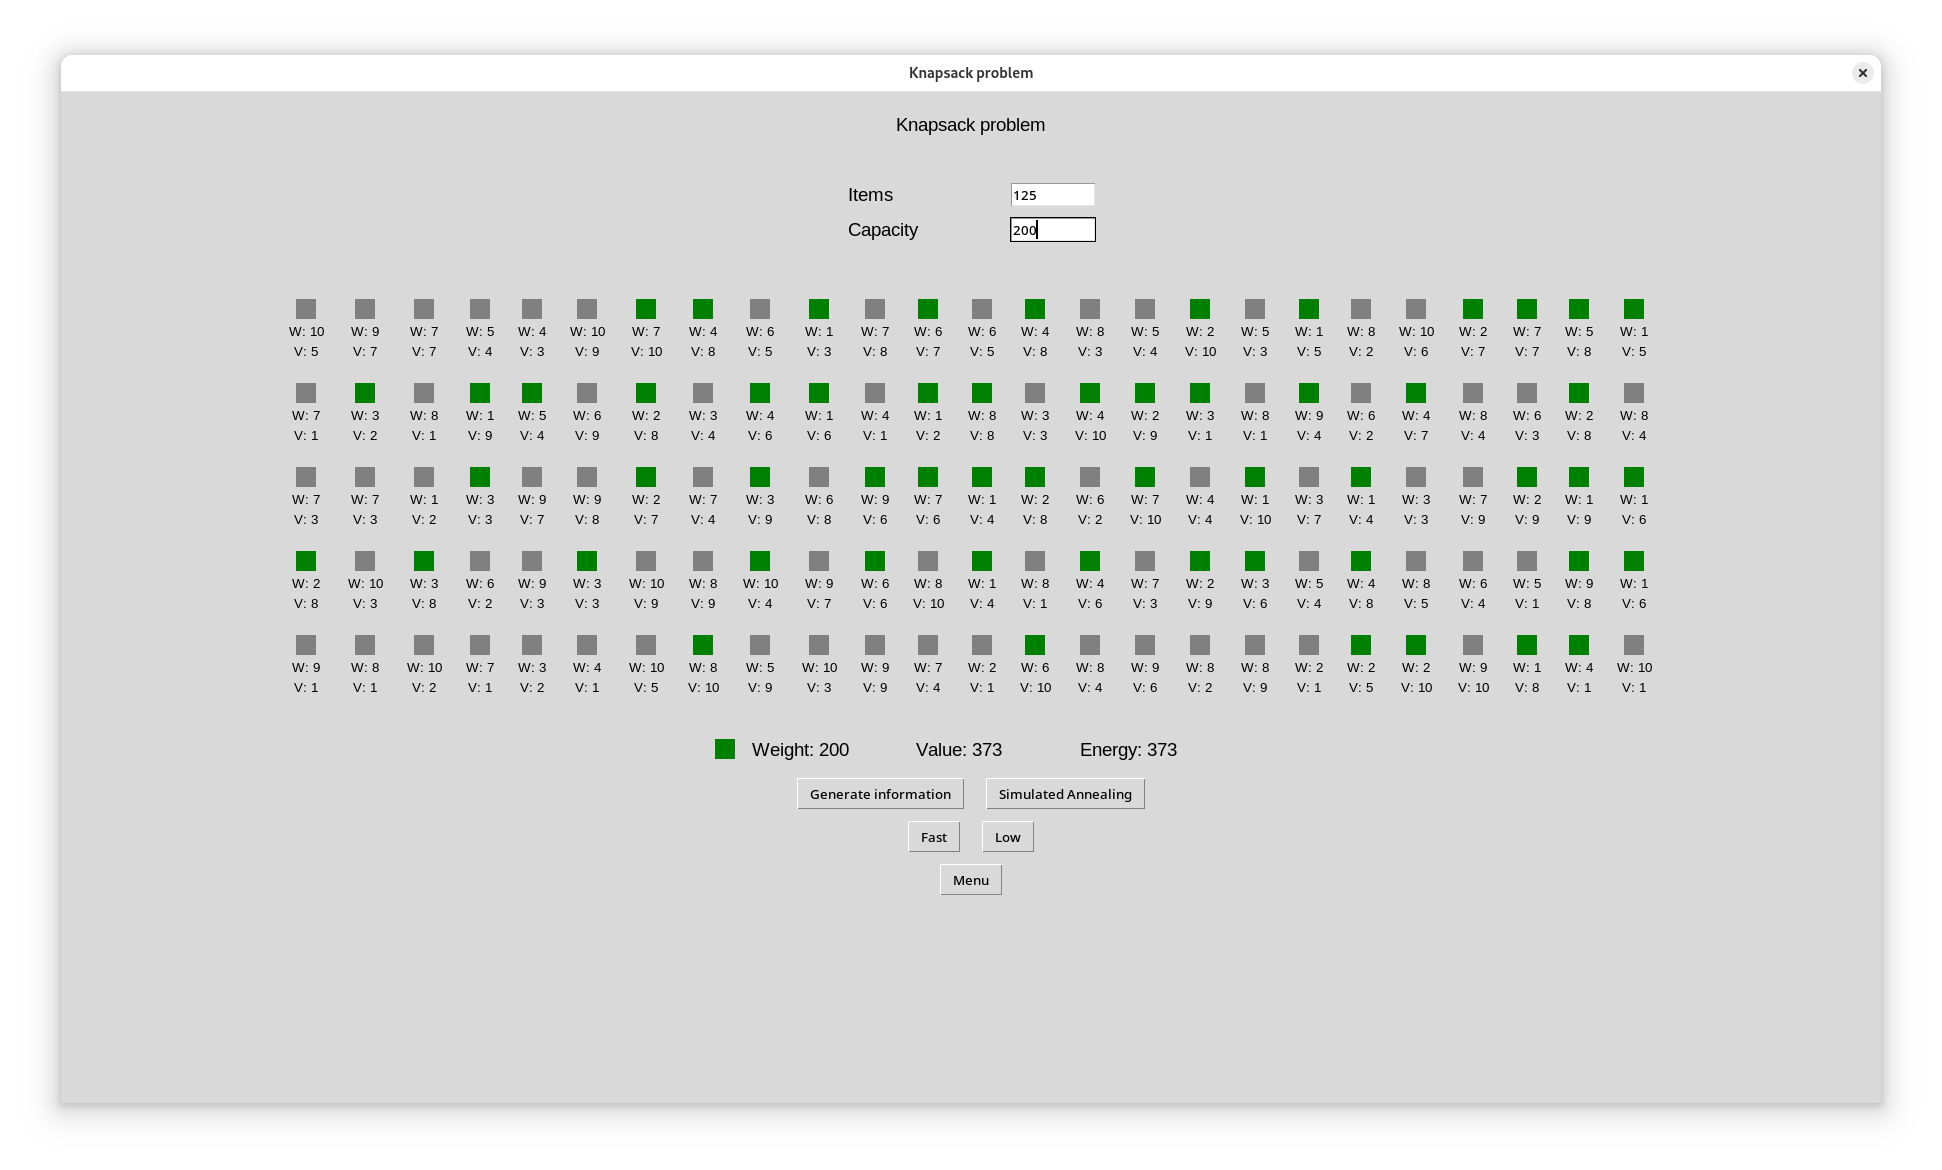
\includegraphics[width=\linewidth]{img/kp}
		\caption{Knapsack Problem Interface}
		\label{fig:kp}
	\end{figure}
	
	
	\subsubsection{Travel Salesman Problem}

La función \ref{lst:tsp-gi} genera una matriz cuadrada y simétrica de $n$ valores aleatorios en un rango de $[1, 100]$.

La función \ref{lst:tsp-e} calcula la energía del sistema. Dado un vector suma todas las distancias de las ciudades con base en la información generada en \ref{lst:tsp-gi}, el resultado que devuelve es negativo ya que se busca minimizar. La función \ref{lst:tsp-gis} genera un vector de $n$ números consecutivos (representando las ciudades) y cambia las posiciones mediante la función \textit{shuffle}.

Finalmente, la función \ref{lst:tsp-rn} toma dos indices aleatorios diferentes e invierte los valores de dichas posiciones del vector.

\begin{lstlisting}[style=pythonstyle, label={lst:tsp-gi} ,caption={Función \textit{generate\_information} de Travel Salesman Problem}]
def generate_information(self, cities):
  distances = [[0]*cities for _ in range(cities)]

  for i in range(cities):
	for j in range(i, cities):  
	  if i == j:
	    valor = 0  
	  else:
		valor = random.randint(1, 100)
	  distances[i][j] = valor
	  distances[j][i] = valor 

  self.information = {
	"cities" : cities,
	"distances" : distances
  }
\end{lstlisting}

\begin{lstlisting}[style=pythonstyle, label={lst:tsp-e} ,caption={Función \textit{energy} de Travel Salesman Problem }]
def energy(self, solution, information):
  distance = 0
  num_cities:int = len(solution)

  for i in range(num_cities):
	current_city = solution[i]
	next_city = solution[(i + 1) % num_cities]  
	distance += information['distances'][current_city][next_city]

  return -distance
\end{lstlisting}

\begin{lstlisting}[style=pythonstyle, label={lst:tsp-gis} ,caption={Función \textit{generate\_initial\_solution} de Travel Salesman Problem}]
def generate_initial_solution(self, information):
  solution =  list(range(information['cities']))
  random.shuffle(solution)
  return solution     
\end{lstlisting}

\begin{lstlisting}[style=pythonstyle, label={lst:tsp-rn} ,caption={Función \textit{random\_neighbour} de Travel Salesman Problem}]
def random_neighbour(self, solution):
  neighbour = solution[:]
  i = j = random.randint(0, len(solution) - 1)
 	while j == i:
	  j = random.randint(0, len(solution) - 1)
  neighbour[i], neighbour[j] = neighbour[j], neighbour[i]

return neighbour
\end{lstlisting}

La interfaz de la figura \ref{fig:tsp} simula 25 ciudades y muestra la exploración de diferentes posibilidades en el espacio de búsqueda. El botón de \textit{distances} muestra la matriz de adyacencia del grafo.

\begin{figure}[h!]
	\centering
	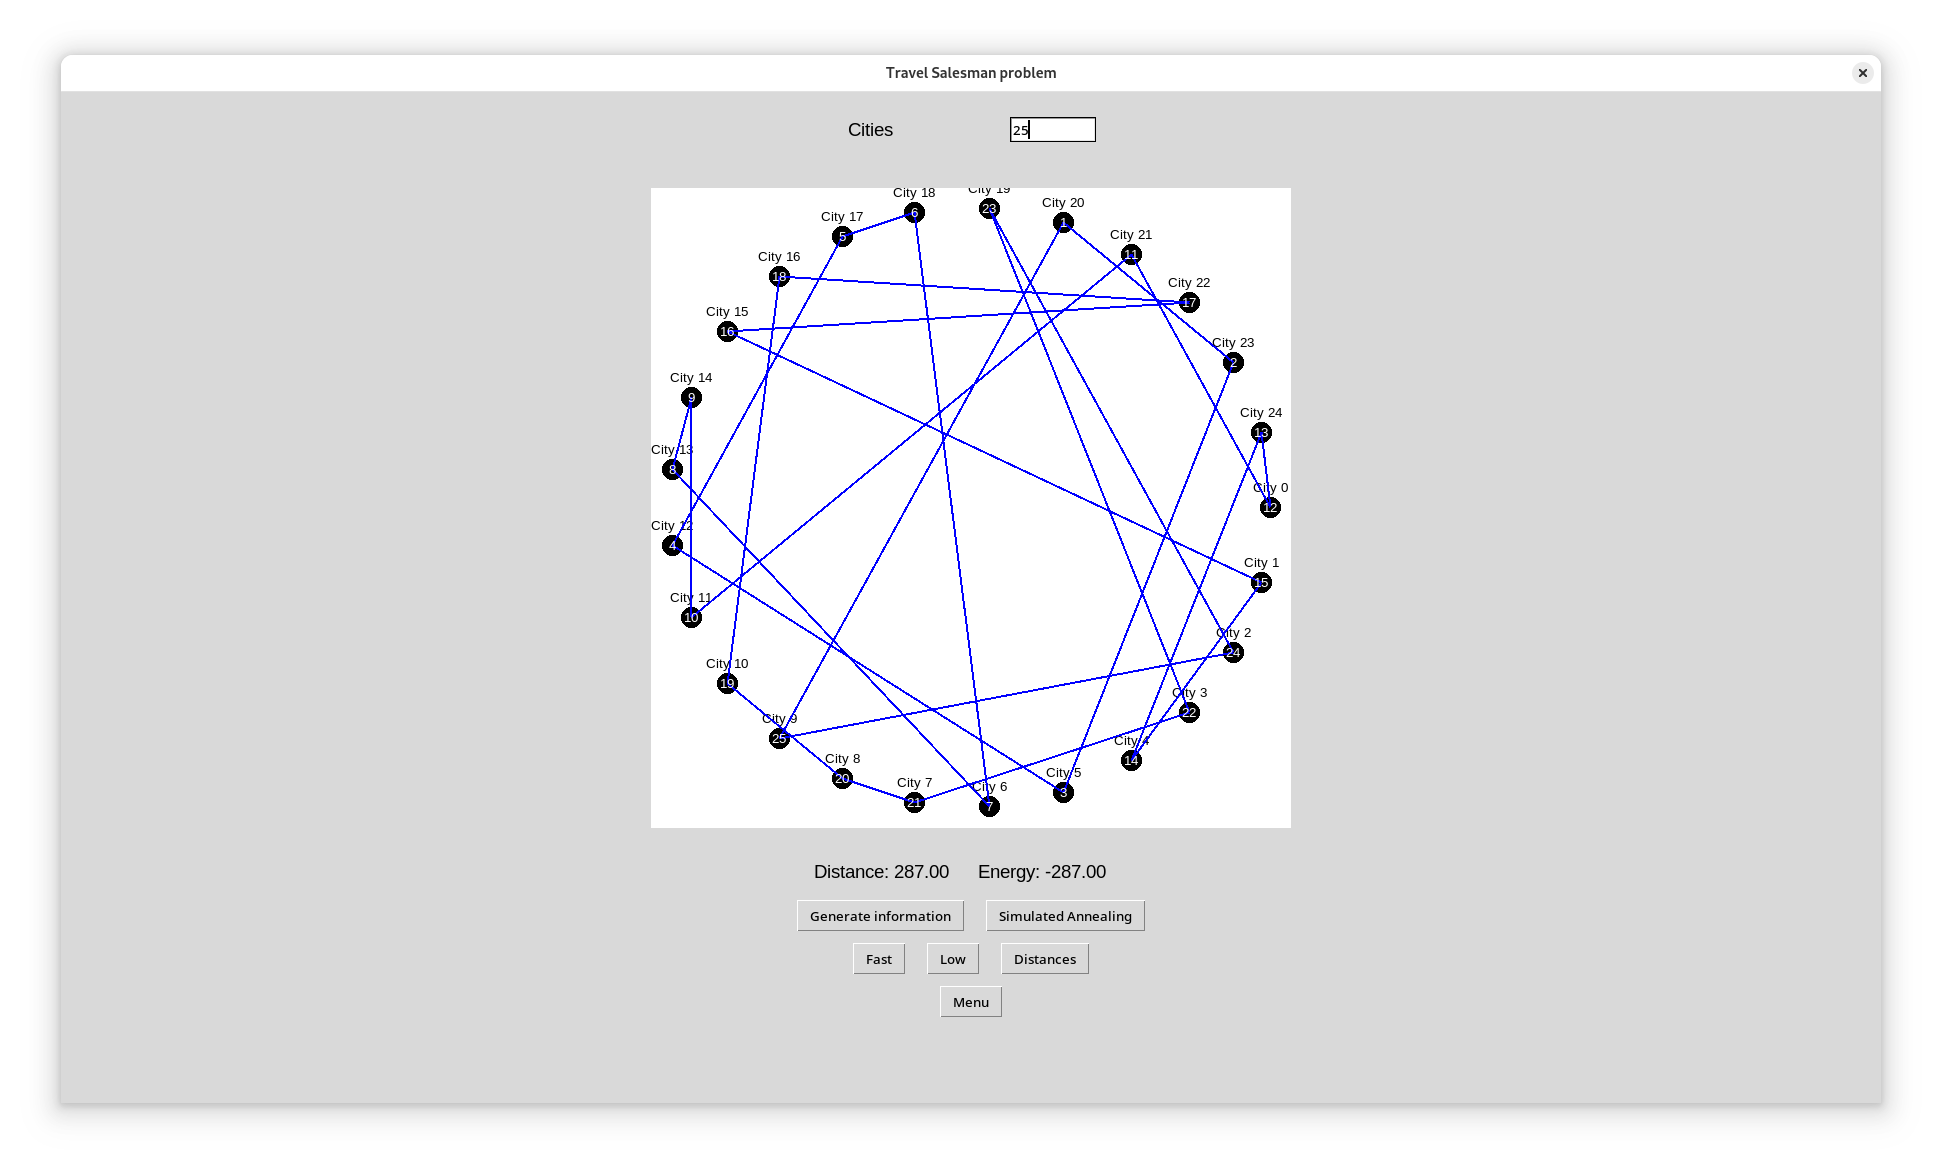
\includegraphics[width=\linewidth]{img/tsp}
	\caption{Travel Salesman Problem Interface}
	\label{fig:tsp}
\end{figure}

	\subsubsection{Minimizar la función}

La función \ref{lst:sfp-gi} unicamente define el tamaño del vector y los rangos de valores. por otro lado, la función \ref{lst:sfp-e} calcula la energía del sistema dada por la suma de los cuadrados, dado que es una función de minimización se invierte el signo.

La función \ref{lst:sfp-gis} genera un vector de $n$ elementos aleatorios en los rangos definidos, mientras que la función \ref{lst:sfp-gn} suma  o resta en uno a un elemento aleatorio del vector (dado que se considera una configuración circular, se ajusta el valor si el nuevo valor no se encuentra en el rango).

\begin{lstlisting}[style=pythonstyle, label={lst:sfp-gi} ,caption={Función \textit{generate\_information} de SumFunctionProblem}]
def generate_information(self, size, min, max):
  self.information = {
	"size": size,
	"min": min,
	"max": max
  }
\end{lstlisting}

\begin{lstlisting}[style=pythonstyle, label={lst:sfp-e} ,caption={Función \textit{energy} de SumFunctionProblem}]
def energy(self, solution, _):
  total_sum:float = 0

  for val in solution:
    total_sum += val**2

  return -total_sum
\end{lstlisting}

\begin{lstlisting}[style=pythonstyle, label={lst:sfp-gis} ,caption={Función \textit{generate\_initial\_solution} de SumFunctionProblem}]
def generate_initial_solution(self, information):
  solution = [random.randint(information['min'], information['max']) for _ in range(information['size'])]
  return solution
\end{lstlisting}

\begin{lstlisting}[style=pythonstyle, label={lst:sfp-gn} ,caption={Función \textit{generate\_neighbour} de SumFunctionProblem}]
def random_neighbour(self, solution):
  neighbour = solution[:]
  index = random.randint(0, len(solution) - 1)
  sign = random.choice([-1 , 1])
  neighbour[index] += sign

  if neighbour[index] > self.information['max']:
	neighbour[index] = self.information['min']

  if neighbour[index] < self.information['min']:
	neighbour[index] = self.information['max']

  return neighbour
\end{lstlisting}

La interfaz de la figura \ref{fig:sfp} simula un vector de 30 elementos en el rango de -10 a 10. Las barras crecen y decrecen según se explore el espacio de búsqueda. 

\begin{figure}[h!]
	\centering
	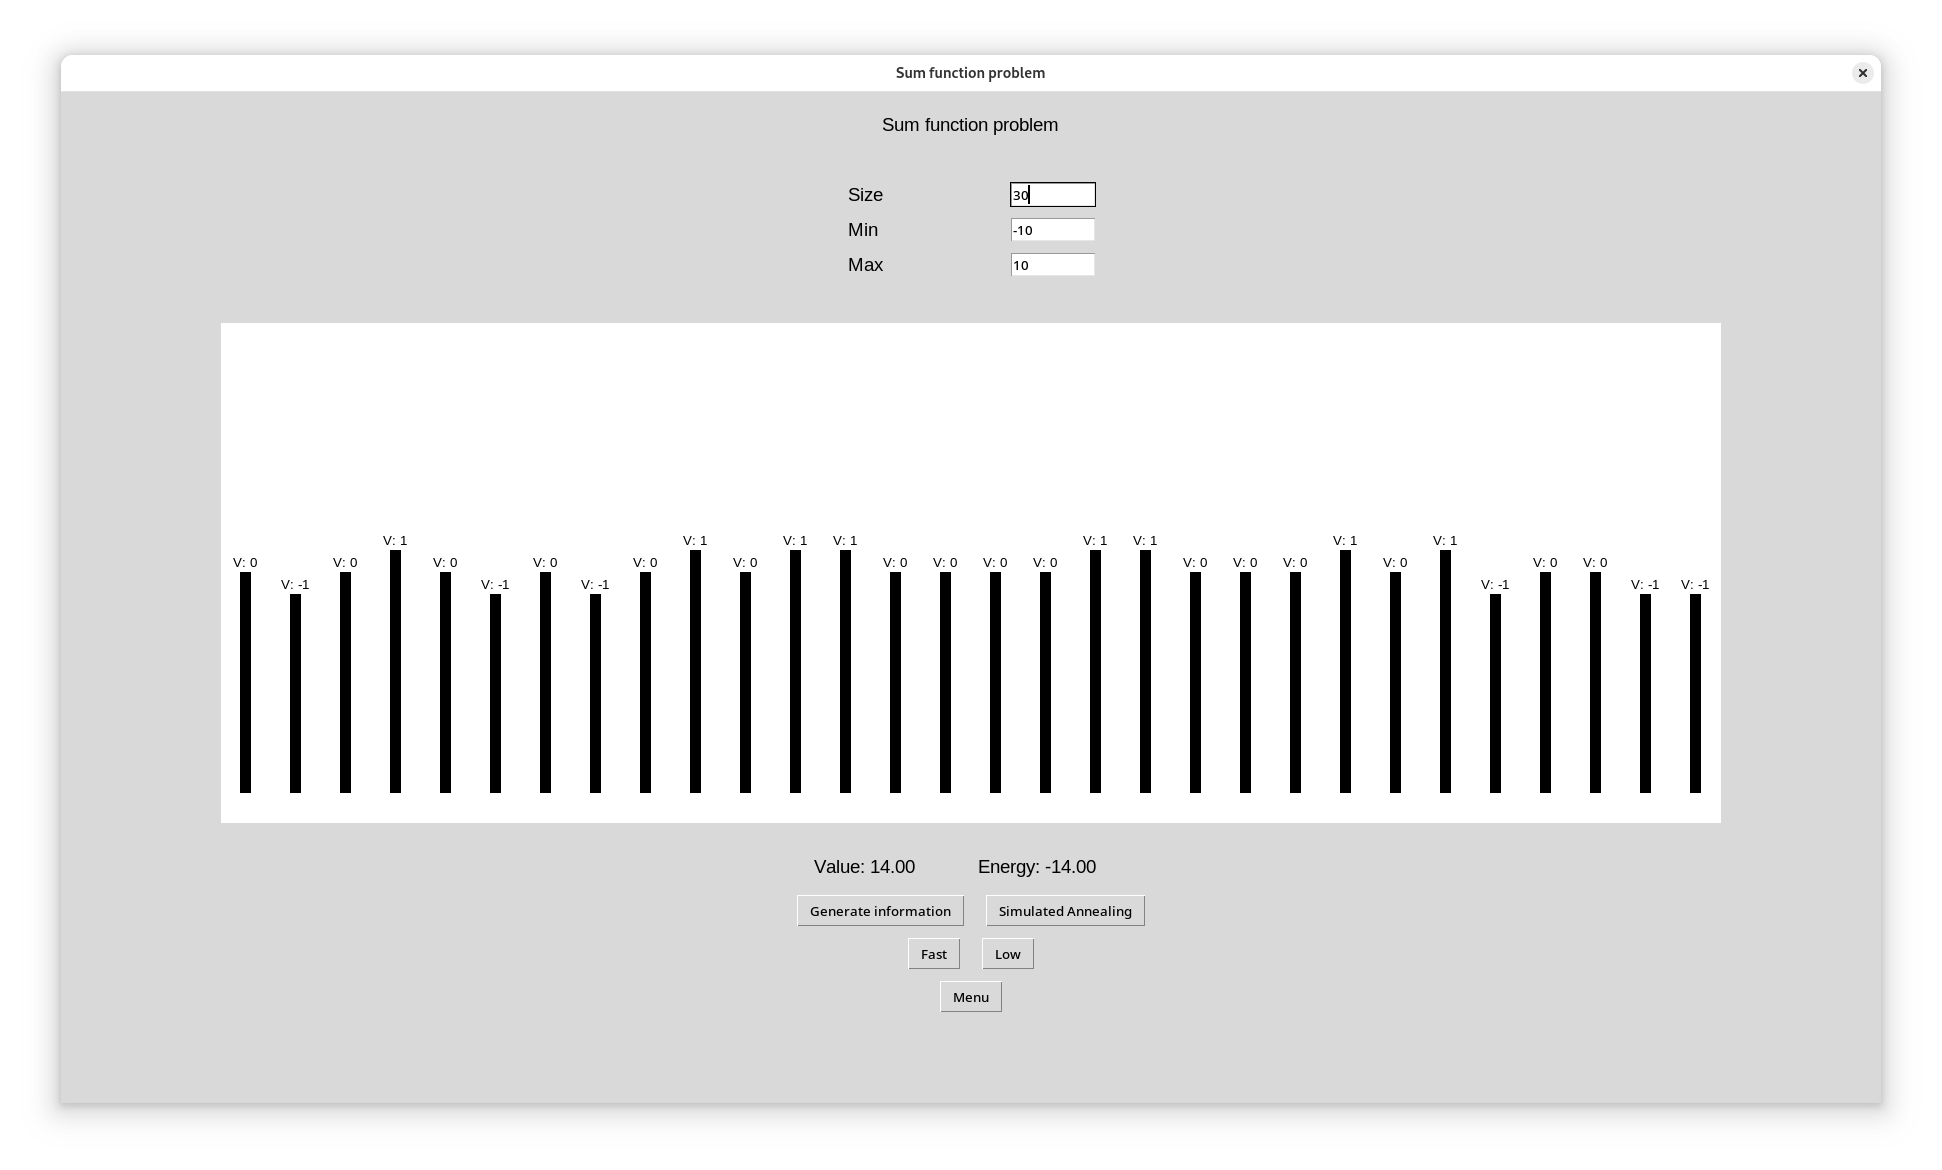
\includegraphics[width=\linewidth]{img/sfp}
	\caption{Sum Function Problem Interface}
	\label{fig:sfp}
\end{figure}

\clearpage
\section{Conclusión}

\textit{Simulated Annealing} tiene muchas mas posibilidades de encontrar un óptimo global pero, de forma redundante se encuentra a su propio problema de optimización el cual consiste en definir los meta parámetros del algoritmo, como la temperatura máxima, mínima, tasa de decrecimiento, etc. Podria resultar interesante aplicar Simulated Annealing para si mismo y analizar la influencia de dichos meta parámetros.

Otro problema es la precisión al momento de encontrar una mejor solución, pues aunque el algoritmo no se haya estancado en alguna posición, si se detiene cuando la temperatura ha superado el umbral establecido.

La implementación de un almacenamiento de los mejores resultados permite registrar si en algún punto se desvío del camino, esto ayudaría a reiniciar el algoritmo pero colocando esa posición como la solución inicial, o incluso, si sabemos que el resultado es próximo, podría optarse por otros métodos como \textit{hill Climbing}, para encontrar una solución mas precisa.


	% Referencias
	\clearpage
	\addcontentsline{toc}{section}{Referencias}
	\bibliographystyle{IEEEtran}
	\bibliography{referencias}

\end{document}
